\chapter{Quantum Optimal Control}\label{chap:3_Quantum_Optimal_control}
\epigraph{``Neo, sooner or later you’re going to realize, just as I did, that there’s a difference between knowing the path and walking the path."}{Morpheus, \emph{The Matrix (1999)}}

The future of quantum technologies depends on our ability to control quantum systems with precision and accuracy. It is a key factor in the realisaton of, for example, quantum computers \cite{ball_software_2021}, communication systems \cite{omran_generation_2019} and quantum sensors \cite{le_robust_2021}, as well as being necessary in the exploration and understanding of fundamental physics. The research field which concerns itself with such control problems is generally known as Quantum Optimal Control Theory (\acrref{QOCT}) \cite{koch_quantum_2022,glaser_training_2015} and its primary objective is the development of techniques which allow for the construction and analysis of strategies, primarily electromagnetic field shapes, that manipulate quantum dynamical processes in the most efficient and effective way possible in order to achieve certain objectives. Common control objectives in the quantum setting can range from state preparation \cite{zhang_when_2019} and quantum gate synthesis \cite{pelegri_high-fidelity_2022}, to protection against decoherence \cite{rooney_decoherence_2012} and entanglement generation \cite{omran_generation_2019}.

While the field of quantum optimal control is vast and would take an entire book to summarize \cite{dalessio_quantum_2016}, this chapter aims to give a broad overview of the topic highlighting its structure, mechanisms, and practical applications, in particular with respect to the methods that are relevant to the rest of the work presented in this thesis. As such, in Sec.~\ref{sec:3.1_structure_quantum_control}, we will begin by exploring the general structure of optimal control problems in detail and showing how an abstract goal can be transformed into a quantitative formula that guides us towards some desired outcome satisfying a given control objective. First, we will discuss the mathematical structure of optimal control problems (Sec.~\ref{sec:3.1.1_mathematical_structure}) followed by an overview and examples of analytical (Sec.~\ref{sec:3.1.2_analytic_optimisation}) and numerical (Sec.~\ref{sec:3.1.3_numerical_optimisation}) methods for finding solutions to said problems, with a focus on methods that will be relevant to the rest of the content in this thesis. Sec.~\ref{sec:3.2_Quantum_optimal_control} will review how optimal control is adapted in the quantum setting and the main idea behind \acrref{QOCT}, while Sec.~\ref{sec:3.3_qoct_methods} will focus on specific methods used for constructing and optimising driving pulses with quantum systems in mind.

\section{The structure of optimal control problems}\label{sec:3.1_structure_quantum_control}

The idea of an optimal control problem is simple: envision a target you want to achieve, cast it into some form of quantitative or abstract mathematical formula and then use this formula to derive the `best' path to get to said objective. There may be many paths to achieve the target and there may be many metrics to determine what `best' means. The aim of the first part of this section is thus to broadly cover the mathematical structure of optimal control problems and to try and convey an idea of what an optimal path \emph{is} and how one might quantify its optimality. Later in the chapter, we will delve more into practical questions of controllability and the process of optimisation, \@i.e.~once an optimal control problem is constructed, how does one go about finding the solution to it. We will cover both analytical methods in Sec.~\ref{sec:3.1.2_analytic_optimisation} and numerical approaches in Sec.~\ref{sec:3.1.3_numerical_optimisation} focusing on a select few optimisation algorithms which will be relevant to further chapters of this thesis. 

\subsection{Mathematical structure}\label{sec:3.1.1_mathematical_structure}

In general, an optimal control problem is composed of a set of state functions $X: \R \rightarrow \R^n$, and a set of time-dependent control functions $U:\R \rightarrow \R^m$ and the optimal control problem consists of finding $x \in X$ and $u \in U$ that minimise some functional $C: X \cross U \rightarrow \R$ such that the constraint
\begin{equation}\label{eq:control_ODE}
    \dot{x} = f(x, u),
\end{equation}
is satisfied almost everywhere. This is a very abstract description and just about any control problem can be expressed as a special case of this formulation \cite{dalessandro_introduction_2021}. To gain more intuition, we can imagine a more concrete example where, \@e.g.~$U$ and $X$ are sets of continuous functions on the interval $[0, \tau]$ satisfying $x(0) = x_0$. In this scenario, $\tau$ could be a time interval during which we want to drive the system from an initial state $x_0$ to a final state $x_f$ using the control function $u(t)$, $t \in [0, \tau]$. The choice of functional $C$ would have to capture the desired outcome of the protocol: that the state of the system after the driving $x(\tau)$ be equal to the target $x_f$. This can be done by choosing a distance metric that depends only on the drive $u$ and is minimised when $x(\tau) = x_f$, \@~e.g.
\begin{equation}\label{eq:example_cost_func}
    C(u) = \norm{x(\tau)  - x_f},
\end{equation}
where $\norm{\cdot}$ represents some norm on the space $X$.

	The functional $C$ is often referred to in literature as the \emph{cost} or \emph{loss} function \cite{wald_statistical_1950} as it encodes the quality of the final protocol with respect to the desired outcome of the protocol. In that sense, we can imagine adding constraints to the problem that may increase the `cost' of the protocol output if they are not satisfied to some degree. For example, Eq.~\eqref{eq:example_cost_func} can be modified to include additional terms:
\begin{equation}\label{eq:example_cost_func2}
    C(u) = \gamma \norm{x(\tau)  - x_f}^2 + \int_0^{\tau} \norm{u(t)}^2 dt,
\end{equation}
where $\gamma$ is a penalty term on the final state that scales its importance relative to the additional second term, which is analogous to the cost in the energy required to achieve the final state. This updated cost function can be read as introducing a competition between the quality of the final state and the amount of energy expended to get it there, mediated by the value of $\gamma$. 

\begin{figure}[t]
\centering
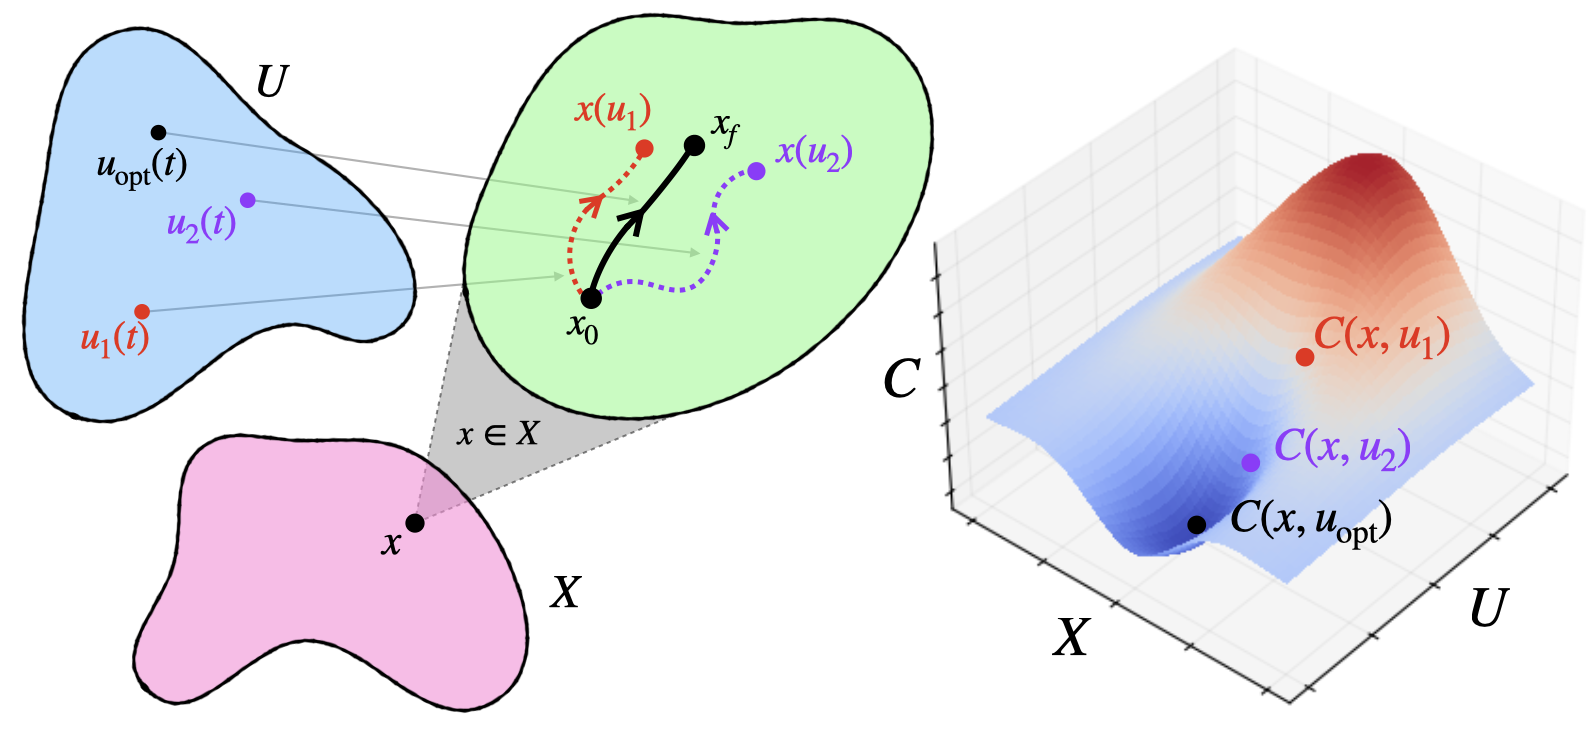
\includegraphics[width=0.9\linewidth]{images/optimal_control_illustration.png} \caption[Illustration of optimal control problem structure]{Illustration of the Mayer type optimal control problem: when an initial value of the system state $x_0$ is fixed, the choice of control function $u \in U$ and the requirement of satisfying Eq.~\eqref{eq:control_ODE} determine $x$ uniquely. The task is then to find $u_{\rm opt}$ such that the functional $C(x, u_{\rm opt})$ is minimised.}\label{fig:optimal_control}
\end{figure}

There are primarily three different types of problem structures in optimal control centering on different constraints and targets: \emph{Mayer-type}, \emph{Lagrange-type} and their combination, \emph{Bolza} problems \cite{dalessandro_introduction_2021}. In this thesis, we will mostly focus on Mayer-type problems, particularly in Ch.~\ref{chap:4_COLD} and Ch.~\ref{chap:6_Applications_fidelity}. In Mayer problems, the initial state is specified $x(0) = x_0$ and the cost function is of the form
\begin{equation}\label{eq:mayer_costfunc}
    C(u) = \phi(x(\tau), \tau),
\end{equation}
with $\phi$ a smooth function and $\tau$ the total time of the protocol. These two constraints and the requirement given by Eq.~\eqref{eq:control_ODE} define the state function $x$ uniquely and the problem is then to determine a control function $u$ on the appropriate set $[0, \tau]$ which minimises Eq.~\eqref{eq:mayer_costfunc}. In Mayer-type problems, a specific target state can be defined in the cost function as a constraint, which is the case in Eq.~\eqref{eq:example_cost_func} and this is illustrated in Fig.~\ref{fig:optimal_control}. However, this need not be the case as target states can be made implicit by having the cost function target some property of the state instead, like Euclidean distance from the initial state in the case of real vectors over Cartesian coordinates. 

From the above, we can view Mayer-type problems as being concerned primarily with the final state of the system and not its path. Lagrange-type problems, on the other hand, put focus on the behaviour of the system throughout the control trajectory and they encompass cost functions of the type
\begin{equation}\label{eq:lagrange_type_costfunc}
    C(u) = \int_0^{\tau} L(x, u, t) dt,
\end{equation}
where $L$ is a smooth function. This type of cost function is applicable, for example, in cases where one wants to minimise the expenditure of some path-dependent resource during the control procedure, or where a path-dependent quantity is easier to optimise over than a target state quantity. This type of optimisation is something that will become relevant in Ch.~\ref{chap:5_cd_as_costfunc} and Ch.~\ref{chap:7_higher_order_agp}. 

The most general type of problem is the Bolza problem, which combines both Mayer and Lagrange in a way that puts emphasis both on the target state of the optimal control and the trajectory that a system takes to get there:
\begin{equation}\label{eq:bolza_tyoe_costfunc}
    C(u) = \phi(x(\tau), \tau) + \int_0^{\tau} L(x, u, t) dt,
\end{equation}
where $\phi$ and $L$ are smooth functions given in Eq.~\eqref{eq:mayer_costfunc} a. A great example of Bolza-type problems is the cost function given by Eq.~\eqref{eq:example_cost_func2}, which comprises a competition between distance to a target state and the energy expended to drive the system to said state. 

Apart from identifying the basic anatomy of control problems in terms of $X$, $U$ and $C$, there is a myriad of additional information about their mathematical structure that can help to analyse and thus solve them. For example, it might be useful to identify if, for a particular optimal control problem, the system in question is \emph{controllable}\cite{dirr_lie_2008, fleming_optimal_1975} \@i.e.~can any initial state be transformed into any desired target state. Equally, it might be useful to study what are called \emph{reachable sets}\cite{vom_ende_reachability_2020, fleming_optimal_1975}, which are sets containing all the states that an initial state can be driven to by the set of control functions $U$. In the case of Mayer-type problems, for example, it might be sensible to define a reachable set parameterised by the final evolution time $\tau$ such that it contains all possible states that can be obtained by the system during a driving time $\tau$. Finally, it would be remiss not to mention the concept of \emph{necessary conditions for optimality}\cite{mangasarian_sufficient_1966}, which focus on determining what formal conditions need to be satisfied for a specific control $u \in U$ to be optimal. Generally, this involves perturbing an assumed optimal control $u$ by some small parameter $\epsilon$ giving $u^{\epsilon}$ and then imposing the constraint that
\begin{equation}\label{eq:optimality_condition}
    C(u^{\epsilon}) - C(u) \geq 0,
\end{equation}
which is then considered the necessary condition for optimality. The most basic of these optimality conditions is the Pontryagin maximum principle or \acrref{PMP} \cite{boltyanski_nonclassical_1999} (see Appendix \ref{app:PMP}), which states that for an optimal control problem, the optimal control and state trajectories should maximize a specific function which combines the system dynamics, the control inputs, and the Lagrange multipliers which encode the constraints of the control problem.

\subsection{Analytical optimisation}\label{sec:3.1.2_analytic_optimisation}

While the first part of optimal control is the construction of the problem, the second part is the search for a solution. The methods used to do this can generally be classified either as analytical or numerical approaches. While both are widely used in optimal control theory, this thesis will largely only focus on the latter, as such we will be brief in introducing the former. 

Analytical optimal control techniques are those that leverage mathematical rigor and formalism to derive solutions or insights, as opposed to relying primarily on numerical simulations, heuristics, or experimentation. They provide a theoretical foundation for understanding the properties and solutions of optimal control problems and are closely related to the discussion in Sec.~\ref{sec:3.1.1_mathematical_structure}. They can allow for a complete geometric understanding of the control problem leading to, for example, knowledge of the structure of a solution or even some proof about a global optimum. For a given set of constraints they might even be used to derive time limits of state transformations, \@i.e.~the concept of reachability. An example of analytical methods is the aforementioned \acrref{PMP}, which provides information about the optimal solution by via a set of differential equations. A different analytical control theory tool, the Hamilton-Jacobi-Bellman equation \cite{yong_dynamic_1999}, provides a way to find the optimal protocol via dynamic programming\cite{sniedovich_dynamic_2010}.

The trouble with analytical approaches, despite the commonplace rigorous guarantees of optimality and the scope of information they provide about the system, trajectory and structure of the control problems and their solutions, is that they are very difficult to scale up and quite inflexible to complex problem constraints. As such, analytical approaches are generally reserved for special cases, when problems have low dimensionality and simple structures where the cost function is generally linear in the arguments. Many real-world control systems require more complexity and flexibility than can be afforded by analytical methods.

\subsection{Numerical optimisation}\label{sec:3.1.3_numerical_optimisation}

To overcome the drawbacks of analytical approaches, many optimal control problems are instead solved using numerical optimisation methods. These are generally algorithmic, iterative  techniques which explore the cost function landscape step-by-step in order to converge to a minimum value. Numerical methods, as a general rule, do not offer the same analysis or guarantees of optimality that analytical methods do. Their iterative nature may lead to a dependence of the outcome on the initial conditions of the algorithm, such as an initial guess for an optimal solution from which the iterations proceed or the bounds on the search space. Despite these drawbacks, however, numerical methods tend to be far more popular than analytical ones simply due to their flexibility and applicability. Where analytical approaches fail, the only way forward is often a numerical method.

A general numerical optimisation technique consists of an initialisation step, a series of search steps and a termination step. These can be summarised as follows:
\begin{enumerate}
    \item \emph{Initialisation}: set up the necessary constraints of the optimal control problem, such as bounds on the solution space or an initial guess for the optimal solution.
    \item \emph{Search}: Perform some iterative search steps (deterministic or stochastic) with the goal of converging to the minimum of the cost function. What constitutes a single step varies massively between different techniques.
    \item \emph{Termination}: Return a solution after some condition is satisfied. This can be a convergence criterion based on the change in the cost function value between steps or a limit on the number of search steps that the algorithm is allowed to perform.
\end{enumerate}

The simplicity of these three components leaves a lot of room for creativity and over the years many numerical optimisation algorithms and techniques have been developed to deal with different constraints and topologies of different cost function landscapes. It would take an entire book \cite{nocedal_numerical_2006} to cover the various categories and subcategories that exist within the field, so we will restrict ourselves to exploring a few key classifications of the structure of numerical optimisation methods. 

One of the more broad ways to classify numerical optimisation methods is into the categories of \emph{gradient-based} methods and \emph{gradient-free} methods. Gradient-based methods, as the name implies, make use of gradient information (the first derivative of the cost function) to guide the search for an optimal solution. These methods are often efficient and converge rapidly when the cost function is smooth and differentiable. A popular example of a gradient-based method is the gradient descent algorithm, which iteratively adjusts the solution in the direction opposite to the gradient, as this direction is likely the steepest decrease in the cost function value. A typical gradient descent protocol might look like:
\begin{equation}\label{eq:gradient_descent}
    \ubb_{n + 1} = \ubb_n - \mu \grad_{\ubb} C(\ubb_n),
\end{equation}
where $n$ denotes the current iteration of the algorithm, $\grad_{\ubb} C(\ubb_n)$ is the derivative of the cost function $C$ with respect to the control parameters $\ubb$ and $\mu$ is generally known as the `learning rate' or `step size' and its job is to control the resolution at which the algorithm traverses the cost landscape. Larger $\mu$ might lead to faster convergence but it might also mean overshooting the cost function minimum, so adjusting its value is often a heuristic that requires some experimentation. Other examples of gradient-based methods include Newton's method and quasi-Newton methods \cite{suli_introduction_2003}, which employ information about the second derivative to guide the search and provide faster convergence as well as a myriad of other approaches including stochastic methods \cite{bottou_tradeoffs_2007}. 

Gradient-free methods, on the other hand, do not require gradient information, making them suitable for optimization problems where the cost function is, \@e.g.~ discontinuous, non-differentiable, or its gradient is difficult or expensive to compute. Examples of gradient-free methods include particle swarm optimization\cite{bonyadi_particle_2017}, the Nelder-Mead method, which we will explore in more detail in Sec.~\ref{sec:3.1.3.1_Nelder_Mead} as well as the Powell method of Sec.~\ref{sec:3.1.3.2_Powell}. These methods often rely on trial and error, random sampling, or mimicking natural phenomena like evolutionary mechanisms\cite{vikhar_evolutionary_2016} to explore the solution space. As in the case of gradient-based approaches, there is a veritable zoo of methods under this umbrella. As the rest of this thesis we will deal almost exclusively with gradient-free methods, we will provide examples of how these techniques look in the next couple of sections.

Apart from the gradient-information, another key way to classify optimisation algorithms is either as \emph{local} or \emph{global}. Local optimization methods are designed to find a local minimum, which is a solution that is better than all other feasible solutions in its vicinity in the landscape of the cost function. They are typically efficient at converging to the local minimum, but they provide no guarantee of finding the global minimum if the cost function is non-convex \@i.e.~the local minimum is not automatically also the global minimum. Both Nelder-Mead and Powell are local methods.

Global optimization methods, on the other hand, aim to find a global optimum, which is the best solution among all feasible solutions, not just those in a local neighborhood. These methods typically employ a strategy to explore the entire solution space, either deterministically or stochastically, to avoid getting trapped in a local optimum. As a result of this larger scope, global optimization methods are generally more computationally intensive than local methods. An example of global optimisation that we will explore in more detail in Sec.~\ref{sec:3.1.3.3_dual_annealing} is Dual-Annealing, which combines generalized simulated annealing\cite{tsallis_generalized_1996}, a global search algorithm, with local optimisers in order to find an optimal solution. Global methods are often used when the optimization problem is complex, non-convex, or the global solution is significantly better than any local solution.

Finally, in numerical optimal control we can make a distinction between open-loop and closed-loop optimisation, particularly when referring to the real-life use or experiments on a given system:
\begin{itemize}
    \item \emph{Open-loop} approaches calculate the control sequence ahead of time and apply it to the system irrespective of the system's actual behavior during the protocol. 
    \item \emph{Closed-loop} methods actively adjust the control strategy based on the current and past states of the system (see Fig.~\ref{fig:quantum_optimal_control}).
\end{itemize}
The closed loop approach is more resilient to uncertainties and disturbances but requires real-time computation or pre-computed feedback laws. In this thesis, the focus will be exclusively on open-loop approaches, as closed-loop methods require access to live experimental data which was not available in the case of the methods explored in later chapters. However, it is important to acknowledge that the results obtained in open-loop optimisations may not reflect the realistic, complex response a physical system might have to a specific control protocol, given that the model we use may not include the full details of the physical system. 

In the following sections we give examples of some common numerical optimisation methods that were used to obtain the results presented in this thesis.

\subsubsection{Nelder-Mead}\label{sec:3.1.3.1_Nelder_Mead}

A frequently used gradient-free optimisers is the Nelder-Mead (or downhill-simplex) method \cite{nelder_simplex_1965} developed by J. Nelder and R. Mead in 1965. It is referred to as a \emph{direct search} or \emph{pattern search} approach and it is a gradient-free local method, making it generally quite efficient, but not guaranteed to converge to a global optimum of the cost function. Direct search methods work by varying each optimisable parameter by some small stepsize from the current minimum in each direction and computing the cost function at the updated value. The change that leads to the largest decrease in the cost function value is taken as the new minimum. Once no such variation leads to an improvement, the stepsize is halved and the process is repeated until some convergence criterion is satisfied.

\begin{figure}[t]
\centering
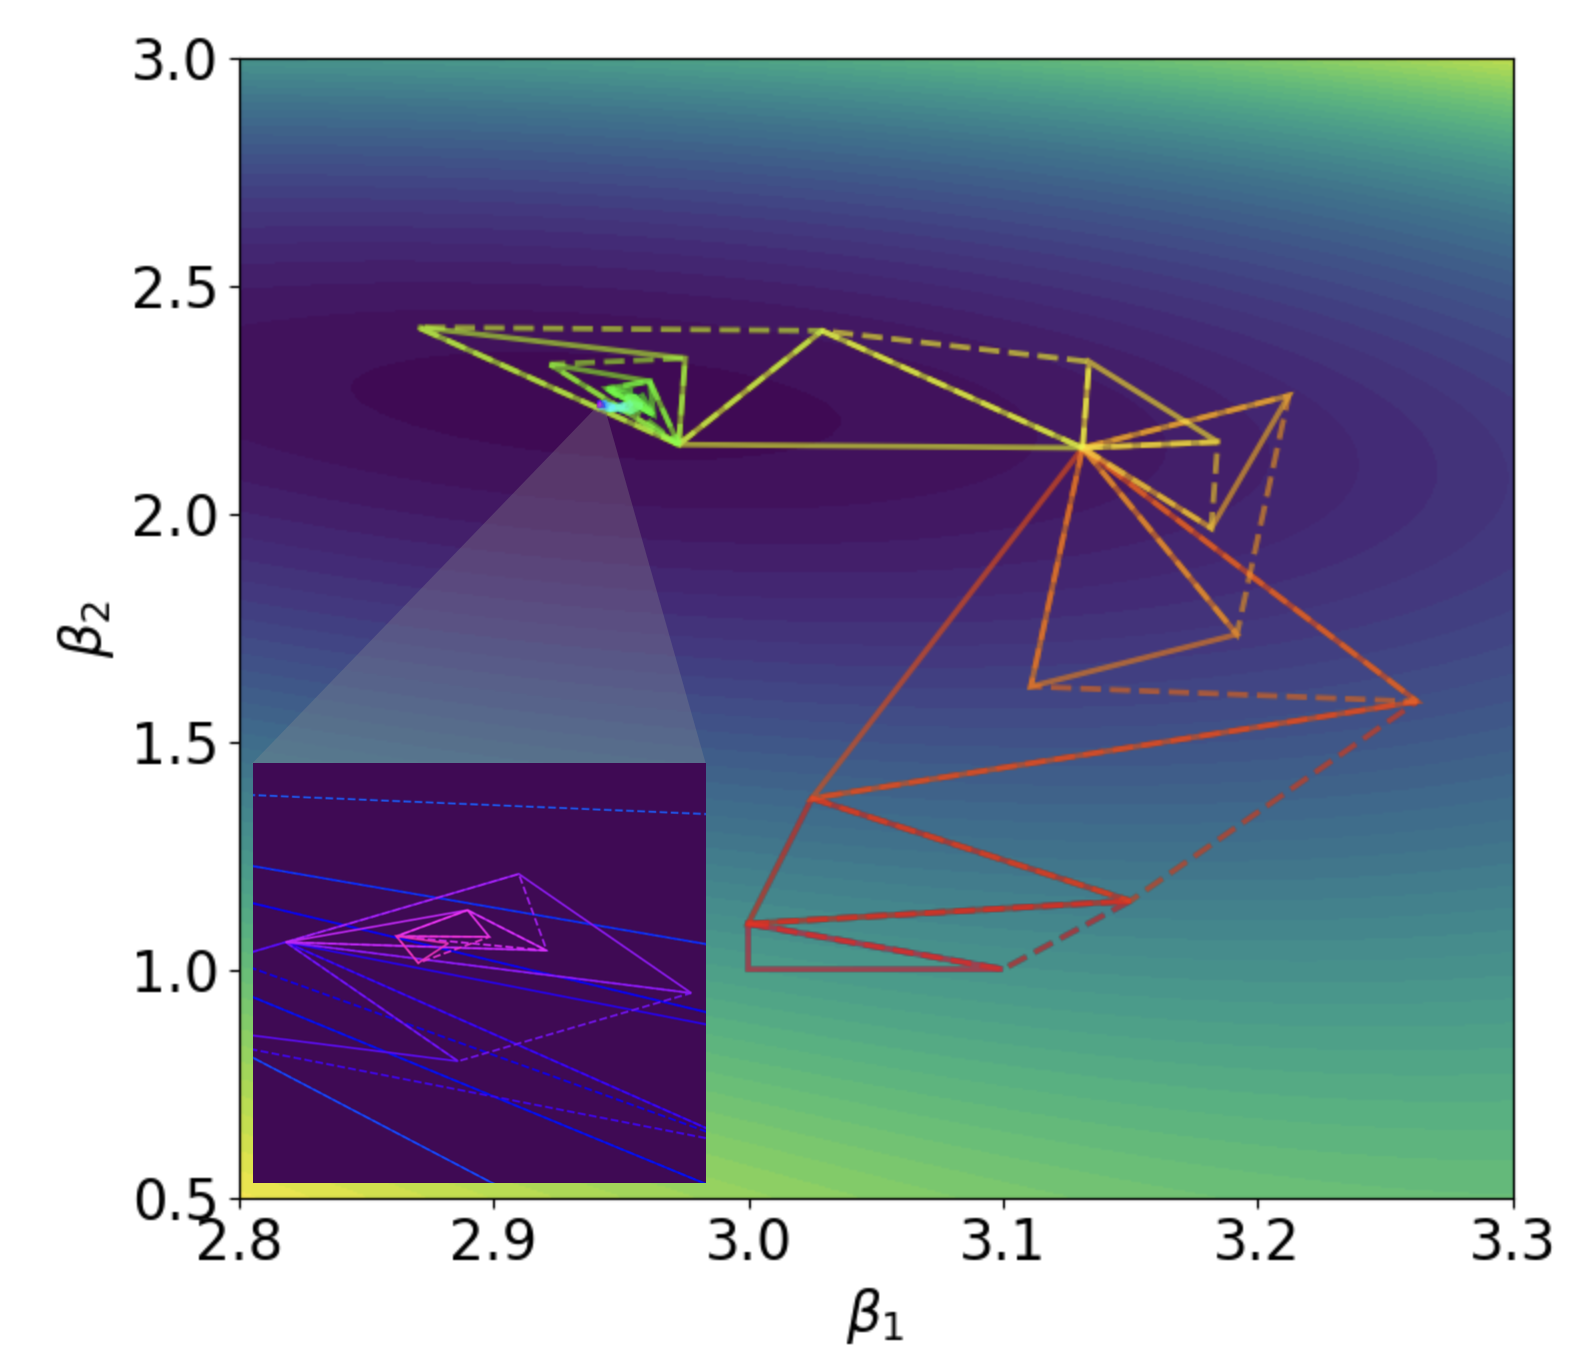
\includegraphics[width=0.6\linewidth]{images/nelder_mead_illustration.png} \caption[Visualising the Nelder-Mead optimisation algorithm.]{Illustration of the Nelder-Mead algorithm for a cost function parameterised by two parameters $\beta_1$ and $\beta_2$. The simplex for a 2-dimensional landscape is a triangle, which then follows the rough algorithm described in the text. The iterations of the algorithm are indicated by constantly switching from solid to dashed edges of the simplex at each step as well as changing in colour. The inset shows a magnification of the final steps of the algorithm.}\label{fig:nelder_mead}
\end{figure}

The way this direct search approach is adapted in Nelder-Mead is by constructing simplices, which are geometric objects that generalise triangles in lower and higher dimensions. For a cost function dependent on $n$ parameters, Nelder-Mead constructs an $n$-dimensional simplex. For $n=0$ this is a point, for $n=1,2,3$ a line segment, triangle and tetrahedron respectively and then higher-dimensional versions as $n$ increases. Thus a simplex has $n+1$ vertices for $n$ parameters. 

The vertices of this simplex then traverse the cost function landscape according to the Nelder-Mead algorithm in order to converge to some minimum value.  In most of the search steps, the primary change is to shift the highest point of the simplex (\@i.e.~where the cost function value is largest) through the opposite face of the simplex, moving to a point with a lower cost function value. These steps are known as \emph{reflections} and they are designed to preserve the volume of the simplex, ensuring it remains non-degenerate. Whenever possible, the method will expand the simplex along a particular direction, which allows it to take bigger steps in search of a minimum. When the simplex encounters a region that can be thought of as a `valley floor' in the cost function landscape, it reduces its dimensions orthogonal to the valley, so that it can slide down. In situations where the simplex has to navigate through a narrow passage, it shrinks itself in all directions, wrapping itself around its best (lowest) point, enabling it to continue its search for the minimum. This process is illustrated for a simple example in Fig.~\ref{fig:nelder_mead}.

This description of the Nelder-Mead method only outlines the basic idea that was first developed in the original 1965 paper. Many variations and improvements have been developed in the years since and the actual implementations. In general, the Nelder-Mead approach is simple to understand and implement, as well as being quite efficient and flexible. However, it often suffers from convergence issues, being both likely to return a sub-optimal local minimum and to get stuck without converging far longer than necessary, undoing any efficiency it otherwise promised. Furthermore, the simplex method doesn't scale well in higher dimensions, making it less effective when the number of parameters is large.

\subsubsection{Powell's method}\label{sec:3.1.3.2_Powell}

Another approach from the gradient-free, local optimiser crowd is Powell's method, first developed by Michael J. D. Powell in 1964 \cite{powell_efficient_1964}. The algorithm is known as a \emph{conjugate-direction} approach, not to be confused with the more common conjugate-gradient approach, although the two are related as the latter can be viewed as a specialisation of the former. 

The basis of Powell's method relies on the idea of conjugate vectors or conjugate directions. Two vectors $\ubb$ and $\boldsymbol{v}$ are said to be conjugate with respect to some positive semi-definite matrix $A$ if $\ubb^T A \boldsymbol{v} = 0$. A set of conjugate directions, thus, is a set of vectors that are pairwise conjugate. Furthermore, one can make the observation \cite{brent_algorithms_2002} that the function
\begin{equation}
    f(\xbb) = \xbb^T A \xbb - 2\boldsymbol{b}^T \xbb + c
\end{equation}
for some positive semidefinite matrix $A$, $\boldsymbol{b} \in \R^n$ and $c \in \R$ has a minimum at the point $\sum_{i=1}^n \beta_i \ubb_i$ in the space spanned by the set of conjugate vectors $\{ u_j \}_{j = 1,...,n}$ with
\begin{equation}
    \beta_i = \frac{\ubb_i^T\boldsymbol{b}}{\ubb_i^T A \ubb_i}.
\end{equation}
This minimum can be calculated efficiently just through evaluating the cost function, without needing explicit access to $A$, $\boldsymbol{b}$ or $c$. This property allowed Powell to develop a simple but powerful gradient-free approach, which can be summarised in the following bit of pseudocode.
\begin{algorithm}
\caption{Powell's Method}
\begin{algorithmic}[1]
\Procedure{Powell}{}
\State Initialise the method with ansatz solution $\ubb_0 \in \R^m$ and $n \leq m$ conjugate search vectors $\{\xbb_1, ..., \xbb_n \}$. If none are provided, use columns of the $m$-dimensional identity matrix.
\For{$i = 1,...,n$}
\State Compute $\beta_i$ to minimise $f(\ubb_{i - 1} + \beta_i \xbb_i)$
\State Define $\ubb_i \gets \ubb_{i - 1} + \beta_i \xbb_i$
\EndFor
\For{$i = 1,...,n-1$}
\State $\xbb_{i} \gets \xbb_{i+1}$
\EndFor
\State $\xbb_n \gets (\ubb_n - \ubb_0)$
\State Compute $\beta$ to minimize $(f(\ubb_0  + \beta \xbb_n))$
\State $\ubb_0 \gets \ubb_0 + \beta \xbb_n$
\EndProcedure
\end{algorithmic}
\end{algorithm}

In other words, the algorithm is initialised with a guess for a solution and a set of conjugate directions. It then proceeds to find a minimum along each direction and shifts to a new point along a superposition of their minima, adding the vector along in which it shifted to the list of conjugate direction vectors and removing the first vector in the list before starting the next step.

\begin{figure}[t]
\centering
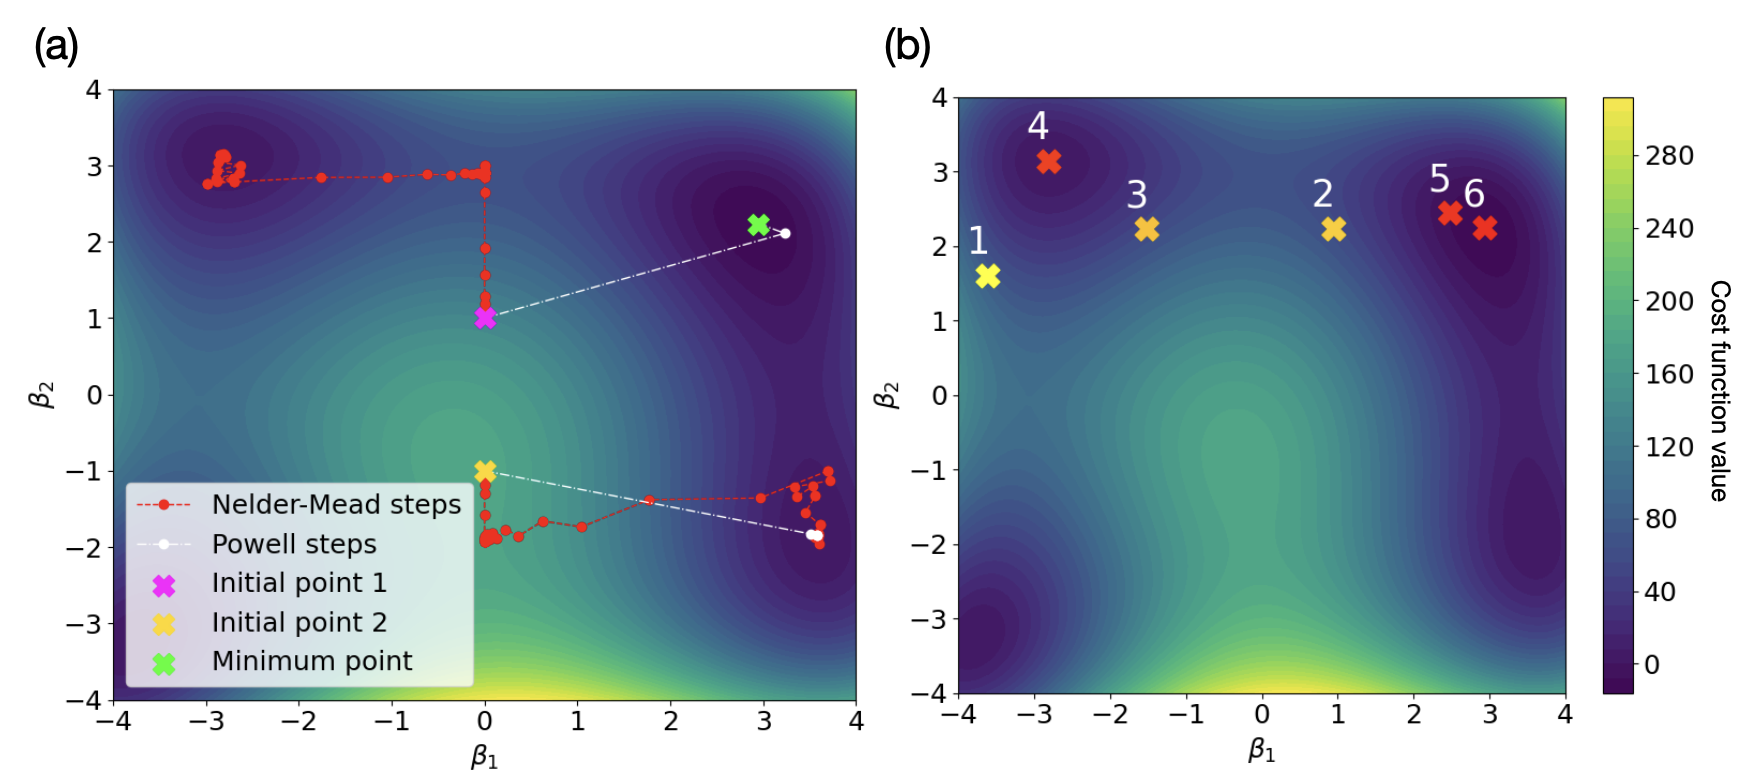
\includegraphics[width=\linewidth]{images/optimiser_plots.png} \caption[Visualising optimisers in action]{An illustration of the optmisation strategy of several numerical optimisation methods. (a) Local optimisers: steps of the Nelder-Mead method and Powell's method when instantiated in two different locations of the loss function landscape. The global mimimum is illustrated by a green cross. (b) The local minima (crosses) visited by the Dual-Annealing in the order indicated by the numbered labels. The colour of the crosses reflects the value of the cost function evaluated at that point as indicated by the colourbar.}\label{fig:optimisers}
\end{figure}

The Powell method is far more complex than is presented here, in particular due to the fact that several extra steps are usually added in order to guarantee convergence and and additional features to help optimise it. Additionally, the minimisation procedure of steps 4 and 11 in the pseudocode is highly non-trivial and can be achieved via several different algorithms like Brent's method\cite{brent_algorithms_2002}. It has guarantees of being very efficient in convex optimisation problems and excels in high-dimensional spaces, unlike Nelder-Mead. A plot of the search steps of the two methods in Fig.~\ref{fig:optimisers}(a) shows how they compare in terms of number of steps taken and accuracy in finding the optimum of some non-convex loss function. Importantly, given the more complicated nature of the steps in Powell's method, the fact that it requires fewer steps to converge to a solution does not necessarily make it more efficient.

\subsubsection{Dual-annealing}\label{sec:3.1.3.3_dual_annealing}

Unlike both Nelder-Mead and Powell's method, dual-annealing is a \emph{global} optimization algorithm, meaning that its primary goal is to find a global minimum of the function. It is also a stochastic method, since rather than follow a pre-defined set of rules or procedures, it employs probabilistic transitions or decisions during the search. This added randomness can help the algorithm escape local optima and explore the solution space more broadly, however it also adds to the computational complexity of such approaches. As mentioned earlier, global optimisation algorithms tend to be far less efficient than local ones, but this is the price that needs to be paid when solutions obtained in local minima are simply not enough and the cost function landscape is highly non-convex. 

What is particularly interesting about dual-annealing is that it combines Generalized Simulated Annealing (\acrref{GSA}) \cite{tsallis_generalized_1996}, a global search algorithm, with a choice of \emph{local} optimiser that refines the solution once the global search is done. This is important because global algorithms, including \acrref{GSA}, are often good at locating the vicinity of the global minimum (the basin) but not necessarily the minimum itself. 

The \acrref{GSA} part of dual-annealing function is, unsurprisingly, a generalisation of the simulated annealing algorithm \cite{kirkpatrick_optimization_1983} inspired by the annealing process of metallurgy which causes a molten metal to reach its crystalline state which is the global minimum in terms of thermodynamic energy. In simulated annealing, the cost function is treated as the energy function of a molten metal and one or more artificial temperatures are introduced and gradually cooled. In \acrref{GSA}, this presents itself as a series of probabilistic jumps across the cost function landscape that depend on an artificial temperature parameter which decreases as the search progresses. 

More concretely, at each step of the search, the algorithm generates a trial jump in the cost function space from the current temporary solution to a new point by sampling it from a modified Cauchy-Lorentz distribution. The distribution peaks around the current temporary solution and its scale parameter (a variable that controls its spread) is a function of the artificial temperature $T_{q_v}$. Thus, the higher the temperature, the more likely it is that the trial jump will be larger. The $q_v$ parameter can be set to different values in order to speed up or slow down the cooling process.

Once the trial jump has been generated, it is either accepted or rejected based on the cost function value at the new point as compared to the current point. If the new point is better (\@i.e.~the jump is `downhill', towards a lower energy), then the jump is accepted. If, on the other hand, the jump is worse or `uphill', it might still be accepted with some probability based on a parameterised Metropolis algorithm \cite{chib_understanding_1995}. This allows for the algorithm to potentially escape local minima. If a jump is accepted, the search then continues in a similar manner from the new point and the temperature parameter is decreased, reducing the probability of the next generated jump being far away from the current point.

The dual-annealing algorithm proceeds by first using \acrref{GSA} to identify a `basin' in the cost function landscape and then using the best solution so far as an initial guess for a local optimisation algorithm like Nelder-Mead or Powell's method to refine the solution. The local search is generally called when the artificial temperature decreases below some pre-defined value and once the local search is done, the whole process restarts again while keeping track of the current best solution. The entire algorithm terminates when some convergence criterion is satisfied. Usually this is when some number of search iterations or cost function evaluations is reached, or there is no more improvement to the solution below some tolerance. This process is illustrated in Fig.~\ref{fig:optimisers}(b), where the dual-annealing algorithm returns points 1, 2 and 4 as minima detected during the annealing stages with 3 and 5 corresponding to minima detected during the local searches. 

The verdict regarding dual-annealing, with respect to the local optimisers that we addressed previously, is that it is far more powerful and can lead to far better solutions, given that it has a far better ability to explore the cost function landscape. However, it is also more computationally expensive, as can be made obvious by the fact that local search is merely a subroutine of the algorithm. Ultimately, the choice of which approach comes down to having knowledge about the cost function landscape as well as trial-and-error. The use of a global optimiser may be overkill when the cost function landscape lends itself well to local methods and each evaluation of the cost function is expensive. If, however, local optimal solutions are not enough, then global methods are by far the best option.

\section{Quantum optimal control}\label{sec:3.2_Quantum_optimal_control}

We've now established that the broad goal of optimal control theory is the design of protocols and strategies which optimise the behaviour of some abstract control system with respect to some abstract target. Quantum optimal control theory (\acrref{QOCT}), rather predictably, does this in the setting where the abstract system is a quantum system. Very broadly then, \acrref{QOCT} concerns itself with the design and analysis of electromagnetic fields that manipulate quantum dynamical processes at the atomic or molecular scale in the best way possible, as illustrated in Fig.~\ref{fig:quantum_optimal_control}. In this chapter, we will broadly cover the basics of \acrref{QOCT}, starting with how the mathematical structure discussed in Sec.~\ref{sec:3.1.1_mathematical_structure} can be adapted to the quantum setting and ending with detailed descriptions of \acrref{CRAB} (Sec.~\ref{sec:3.3.1_CRAB}) and \acrref{GRAPE} (Sec.~\ref{sec:3.3.2_GRAPE}), popular \acrref{QOCT} methods which will be relevant to later work presented in this thesis. As the content of later chapters will focus on closed systems, that will be the perspective we will take with respect to \acrref{QOCT}. More concretely, we will focus on cases where the generator of transformations of a quantum system is primarily modelled as the Hamiltonian as opposed to, \@e.g.~a Liouvillian, but a similar analysis holds in the case of open systems which are just as interesting, if not quite as relevant to this thesis.

Returning to the material covered in Sec.~\ref{sec:3.1.1_mathematical_structure}, we can now add more structure to the abstract notions of system, control function and cost function. In the quantum setting, the set of state functions $X$ often takes the form of a set of quantum states, be they complex vectors, density matrices or operators. The set of control functions $U$ is usually represented by a set of functions of parameterised Hamiltonians. It is common to decompose a control Hamiltonian into two components: the time-dependent `drive' part and the time-independent `drift' part. The time-dependent part can then be further decomposed into a set of $N_k$ operators $\{\mathcal{O}_{\rm opt}^{(k)}\}_{k=1,...,N_k}$, such that the full control Hamiltonian reads:
\begin{equation}\label{eq:optimal_control_H}
    H(\ubb(t)) = H_0 + \sum_{k = 1}^{N_k} u_k(t) \mathcal{O}_{\rm opt}^{(k)},
\end{equation}
where $H_0$ is the drift Hamiltonian with no external controls and the control functions $u_k(t) \in \ubb(t)$ drive the corresponding operators $\mathcal{O}_{\rm opt}^{(k)}$.

\begin{figure}[t]
\centering
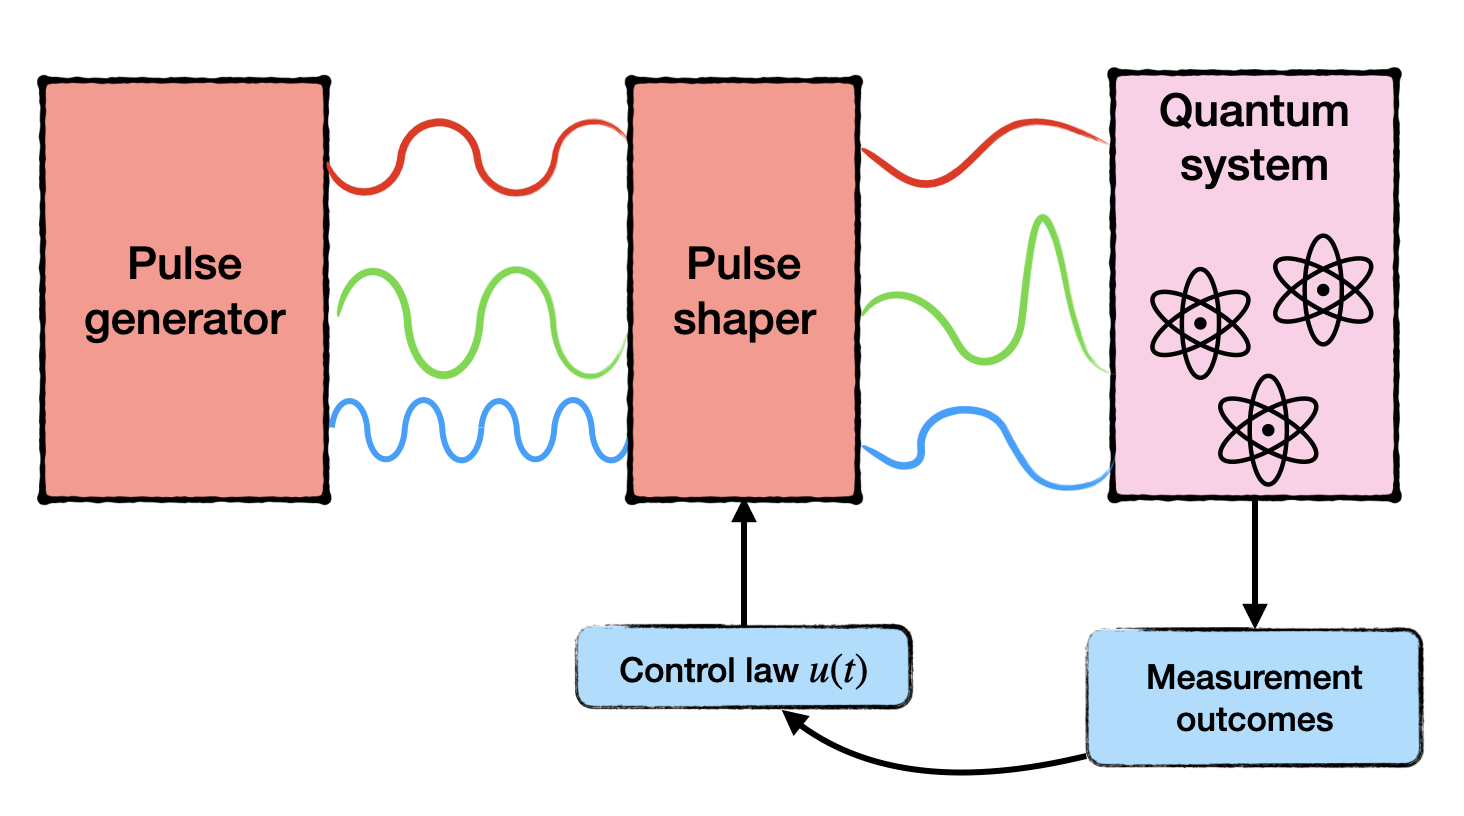
\includegraphics[width=0.8\linewidth]{images/optimal_control_placeholder.png} \caption[Schematic diagram of open-loop quantum optimal control]{A sketch of a quantum optimal control closed-loop set-up. A quantum system is directly controlled by a set of electromagnetic pulses which are shaped according to a set of control functions $\ubb(t)$ that are optimised based on feedback from the information obtained through measurements of the system.}\label{fig:quantum_optimal_control}
\end{figure}

Given this, we can describe a general quantum optimal control problem in analogy to Eq.~\eqref{eq:control_ODE} as one where the aim is to solve the Schr\"{o}dinger equation:
\begin{equation}\label{eq:optimal_control_schroedinger}
    i \hbar \partial_t \ket{\psi(t)} = H(\ubb(t))\ket{\psi(t)},
\end{equation}
with the constraint of starting in a state from a set of initial states $\ket{\psi_0} \in \boldsymbol \Psi_0$ and while minimising some cost function that targets a set of final states $\ket{\psi_T} \in \boldsymbol \Psi_T$. We note that while we are using wavefunctions as representations for the states of the control system, it is actually quite common in \acrref{QOCT} to instead work in the operator picture, where the Schr\"{o}dinger equation is
\begin{equation}\label{eq:operator_schroedinger_eq}
    \partial_t \mathcal{O}(t) = -i H(\ubb(t))\mathcal{O}(t),
\end{equation}
where $\mathcal{O}$ is an operator on some pre-defined Hilbert space. A useful constraint in this setting is to take the initial state of the operator to be the identity $\mathcal{O}(0) = \mathds{1}$. The choice of wave mechanics or matrix mechanics depends on the specific \acrref{QOCT} problem at hand, although questions of \@e.g.~controllability are usually best-solved with operators rather than state vectors. For example, if we can show that the set of possible matrices that can be obtained for system \eqref{eq:operator_schroedinger_eq} is the set of all the unitary matrices (with the rank of the system Hilbert space), then the system can theoretically be steered to any arbitrary state and thus it is controllable.

The choice of cost function in the quantum setting is generally informed by the desired properties of the target state(s) combined with considerations for what information can be extracted from the system and other constraints. For example, when the aim of the optimisation is to prepare a single, well-defined quantum state $\ket{\psi_T}$ with high accuracy, then the most informative cost function is:
\begin{equation}\label{eq:costfunc_fidelity}
    C_{\rm F}(\tau, \ubb) = 1 - F(\tau, \ubb) = 1 - \abs{\braket{\psi(\tau, \ubb)}{\psi_T}}^2,
\end{equation}
where $F(\tau, \ubb)$ is the fidelity of the final state $\ket{\psi(\tau, \ubb)}$ with respect to the desired target $\ket{\psi_T}$. Here $\ket{\psi(\tau, \ubb)}$ is generated by driving an initial state $\ket{\psi_0} \in \boldsymbol \Psi_0$ for a time $\tau$ via the time-dependent Hamiltonian $H(\ubb(t))$. If, on the other hand, the target state need only be a ground state of some Hamiltonian $H_T$, then it might be far more convenient to use the final system energy:
\begin{equation}\label{eq:costfunc_energy}
    C_{\rm E}(\tau, \ubb) = \mel{\psi(\tau, \ubb)}{H_T}{\psi(\tau, \ubb)}.
\end{equation}
Finally, should one be interested only in a specific property of the final state, like its entanglement, then the cost function might look something like:
\begin{equation}\label{eq:costfunc_entanglement}
    C_{\rm S}(\tau, \ubb) = -S[\ket{\psi(\tau, \ubb)}],
\end{equation}
where $S[\cdot]$ is some appropriate measure of entanglement. As well as being informed by the set of target states, the cost function may include further constraints, like the total power of the driving fields in the Hamiltonian. This is analogous to the cost function in Eq.~\eqref{eq:example_cost_func2}, which in the quantum case might look something like:
\begin{equation}\label{eq:costfunc_constraint}
    C(\tau, \ubb) = C_{\rm F}(\tau, \ubb) + \sum_{k = 1}^{N_k} \int_0^{\tau} \abs{u_k(t)}^2 dt,
\end{equation}
which can be read as an optimisation for final state fidelity with the added constraint that the time-integrated flux of the driving fields is minimised. 

\section{Quantum optimal control methods}\label{sec:3.3_qoct_methods}

Both analytical (Sec.~\ref{sec:3.1.2_analytic_optimisation}) and numerical (Sec.~\ref{sec:3.1.3_numerical_optimisation}) methods have been developed for the optimal control of quantum systems in recent decades. Analytical methods in \acrref{QOCT} generally deal with questions of necessary conditions for controllability \cite{schirmer_complete_2001} or reachability of states, \@e.g.~exploring quantum speed limits \cite{khaneja_time_2001, hegerfeldt_driving_2013, poggi_quantum_2013}. Analytical methods \emph{can} be used to find solutions to quantum optimal control problems rather than just classify their structure, but the Achilles' heel of analytical approaches remains a general inability to deal with complex systems. The volatile and often exponentially complex nature of quantum systems means that numerical approaches tend to be the preferred method for actually determining solutions to \acrref{QOCT} problems. 

Numerical methods in \acrref{QOCT} tend to consist of the development and analysis of iterative algorithms focused on optimising pulses for quantum systems. This can be done by constructing a mathematical description of the pulse, including parameters that control its shape and which can then be numerically optimised. Most numerical methods under the umbrella of \acrref{QOCT} involve a classical optimiser, like those discussed in Sec.~\ref{sec:3.1.3_numerical_optimisation}, as a subroutine in the approach which finds the optimal values for the pulse parameters. In this section we will explore two of the more broadly used numerical approaches in quantum optimal control, \acrref{CRAB} and \acrref{GRAPE}. 

\subsection{Chopped random-basis quantum optimization (CRAB)}\label{sec:3.3.1_CRAB}

The ``Chopped random-basis quantum optimization" or \acrref{CRAB} method is a quantum optimal control method first introduced in \cite{doria_optimal_2011, caneva_chopped_2011} which revolves around the construction of a truncated randomized basis of functions for the control fields of a quantum system. It was originally developed for quantum many-body systems whose time evolution can be efficiently simulated by time-dependent density matrix renormalization group (tDMRG)\cite{white_density_1992, schollwock_density-matrix_2005, schollwock_density-matrix_2011}. It was believed that such systems were mostly intractable for control optimization using gradient-based algorithms \cite{brif_control_2010}, although such potential limitations have been overcome in more recent work\cite{jensen_approximate_2021}. \acrref{CRAB} provides a way to reduce the space of search parameters, making the optimisation process more efficient, while retaining access to a large solution space through the added randomisation component.

The key idea is to expand the control pulse $\ubb(t)$ in some truncated basis of dimension $N_k$: 
\begin{equation}\label{eq:basic_CRAB}
    u(t) = \sum_{i = 1}^{N_k} c_i u_i(t),
\end{equation}
where the cost function landscape is spanned by the coefficients $c_i$, that need to be optimised over using numerical optimisation methods like those described in Sec.~\ref{sec:3.1.3_numerical_optimisation}. Generally this basis is made up of trigonometric functions although it could be any basis that spans the space of admissible controls \@e.g.~generalized Chebyshev polynomials. A choice of basis can further be enhanced or modified by a shape function $g(t)$ that fixes the pulse to some initial and/or final value:
\begin{equation}\label{eq:trigonometric_CRAB}
    u(g(t),t) = \sum_{i = 1}^{N_k/2} c_i \frac{\cos{\omega_i t}}{g(t)} + \sum_{i = N_k/2 + 1}^{N_k} c_i \frac{\sin{\omega_i} t}{g(t)}.
\end{equation}

Importantly, the key to expanding the solution space in order to find better pulses using the \acrref{CRAB} approach lies in the randomisation of the frequencies $\omega_i$. During each optimisation process, the $\omega_i$ are chosen randomly around the principal harmonics within some interval $[0, \omega_{\rm max}]$, allowing the pulse shapes to be more diverse and more complex than by simply keeping them fixed at a certain value. The optimisation process can then be parallelised, with several optimisation instances running simultaneously exploring several different sets of random frequencies and the optimal solution can be picked from the final outcomes of all optimisations. 

The \acrref{CRAB} approach lends itself very easily to the incorporation of additional features and constraints like the shape function. For example, it is quite easy to start with a trial pulse, say $f(t)$, which cannot be expanded efficiently or exactly in the chosen basis and to dress it according to
\begin{equation}\label{eq:trial_pulse_CRAB}
    u(t) = f(t)\Bigg(1 + \sum_{i = 1}^{N_k} c_i u_i(t)\Bigg).
\end{equation}
Another particularly useful alteration to the basic \acrref{CRAB} procedure is what is known as `dressed' \acrref{CRAB} or dCRAB \cite{rach_dressing_2015}, which in a similar vein aims to iteratively re-dress solutions obtained from previous optimisations with new sets of basis functions added onto the existing solution. These \emph{super-iterations} $j$ can be modelled as
\begin{equation}\label{eq:dCRAB}
    u^j(t) = c_0^j u^{j-1}(t) + \sum_{i = 1}^{N_k} c_i^j u^j_i(t),
\end{equation}
where $u^j_i(t)$ are new basis functions and $u^{j-1}(t)$ is the pulse obtained from a previous, $(j-1)^{\rm st}$ optimisation. The coefficient $c_0^j$ can be seen as shifting the solution in the direction of the previous solution pulse while $\{ c_i^j\}_{i = 1, ..., N_k}$ move it in new search directions $u^j_i(t)$. This is, in fact, very similar to Powell's optimisation method which we covered in Sec.~\ref{sec:3.1.3.2_Powell}, wherein a finite set of search directions in cost function space is continuously updated with linear combinations of their optima. dCRAB can be seen as doing the same but with updates sampled from an infinite-dimensional search space. This iterative approach is useful in  avoiding local minima and in exploring a far larger search space, avoiding the hard constraint of a finite set of basis functions for each optimisation. 

There are several key advantages in the \acrref{CRAB} approach that have led to its widespread use in the \acrref{QOCT} community. For one, the randomization of the control field basis allows for a more comprehensive exploration of the control landscape, which can lead to the discovery of better solutions. It also offers relatively quick convergence as the number of optimisable parameters is usually small when compared to other approaches (such as \acrref{GRAPE}, which we will explore in the next section). Finally, it is very flexible: the basis functions can be altered and constraints can be incorporated quite easily, whether they concern the physical implementation (\@e.g.~the shaping function) or the efficiency of the optimisation itself.

\subsection{Gradient Ascent Pulse Engineering (GRAPE)}\label{sec:3.3.2_GRAPE}

The ``Gradient Ascent Pulse Engineering" (GRAPE) algorithm is yet another widely used \acrref{QOCT} numerical method. It was first developed in order to design pulse sequences in NMR spectroscopy \cite{khaneja_optimal_2005} and has since been iterated upon and improved a number of times as well as being integrated into several optimal control packages \cite{de_fouquieres_second_2011, chen_iterative_2022, machnes_comparing_2011, johansson_qutip_2013}. As the name suggests, it is a gradient-based optimisation method and while initially it was used primarily for the preparation of specific target states, its powerful flexubility has since lent itself to many other applications in the setting of quantum technologies, like the optimisation of quantum logic gates \cite{motzoi_optimal_2011, anderson_accurate_2015}.

The key idea behind \acrref{GRAPE} is to replace continuous control functions, like \@e.g.~those used in the basis functions of \acrref{CRAB}, with piecewise constant control amplitudes $u_j(t_k)$, each applied to the control system at time $t_k \in [0, \tau]$ for a time interval $\Delta t$, where $\tau$ is the total evolution time. You can view this as discretizing the time-evolution of the system into $N_m$ slices of time $\Delta t = t_{k + 1} - t_k$. These slices need not all be of equal size, but for simplicity let us work in the setting where they are, meaning that $\tau = N_m \Delta t$.

At this point we can pause and notice that since the control amplitudes $u_j(t_k)$ are piecewise constant for all time intervals, they can be treated as a set of parameters that can be optimised using a numerical optimisation algorithm. This gives $N_j \cross N_m$ total parameters to optimise, as each $j^{\rm th}$ pulse will be made up of $N_m$ time-steps. Given this relatively large number of parameters, the original \acrref{GRAPE} algorithm included an analysis of how to compute the gradient of the cost function with respect to each $u_j(t_k)$ in order to implement gradient-based optimisation methods like gradient-descent (Eq.~\eqref{eq:gradient_descent}). Recalling the form of the quantum control Hamiltonian from Eq.~\eqref{eq:optimal_control_H}, the propagator for the time-evolution of the quantum system using \acrref{GRAPE} during a single time step $\Delta t$ at time $t_k$ is
\begin{equation}
    U_k(\Delta t) = \exp{- i \Delta t \Big( H_0 + \sum_{j=1}^{N_j} u_j(t_k) \mathcal{O}_{\rm opt}^{(j)} \Big)}
\end{equation}
for some drift component of the Hamiltonian $H_0$ and some basis of control operators $\{\mathcal{O}_{\rm opt}^{(j)}\}_{j = 1,...,N_j}$. The full evolution of the system can thus be captured by the product of operators (with dependence on $\Delta t$ removed):
\begin{equation}
    U(\tau) = U_{N_m} U_{N_m - 1} ... U_{2} U_{1},
\end{equation}
such that for some initial state $\rho_0$ (where we are now working with density matrices rather than state vectors), the final evolved state can be written as
\begin{equation}\label{eq:grape_rho_evolved}
    \begin{aligned}
        \rho(\tau) &= U(\tau)\rho_0 \adj{U}(\tau) \\
        &= U_{N_m} ... U_{1} \rho_0 \adj{U}_{1} ... \adj{U}_{N_m}
    \end{aligned}
\end{equation}

In order to derive a way to compute the gradient of the cost function with respect to the parameters, it is necessary to define a cost function. In this case we will use the overlap of the final state $\rho(\tau)$ with respect to some target state $\rho_T$, a density matrix version of Eq.~\ref{eq:costfunc_fidelity}:
\begin{equation}
    C(\ubb) = \Tr{\rho_T^{\dagger}\rho(\tau)},
\end{equation}
where $\ubb$ in this case is the set of all $N_j \cross N_m$ parameters to be optimised $\ubb: \{ u_j(t_k)\}_{j = 1, ..., N_j}^{k = 1,...,N_m}$. Using Eq.~\ref{eq:grape_rho_evolved} and the cyclic property of the trace we can write
\begin{equation}\label{eq:grape_costfunc_rewrite}
    \begin{aligned}
        C(\ubb ) &= \Tr{\rho_T^{\dagger}U_{N_m} ... U_{1} \rho_0 \adj{U}_{1} ... \adj{U}_{N_m}} \\
        &=  \Tr{\adj{U}_{k+1} ... \adj{U}_{N_m} \rho_T U_{N_m} ... _{k+1} U_{k} ... U_{1} \rho_0 \adj{U}_{1} ... \adj{U}_{j}} \\
        &= \Tr{\Lambda_k \rho_k},
    \end{aligned}
\end{equation}
where $\Lambda_k = \adj{U}_{k+1} ... \adj{U}_{N_m} \rho_T U_{N_m} ... _{k+1}$ and $\rho_k = U_{k} ... U_{1} \rho_0 \adj{U}_{1} ... \adj{U}_{j}$. 

In order to calculate the gradient of $C(\ubb)$ with respect to each parameter $u_j(t_k)$, we first investigate what happens to $U_k$ when we perturb each parameter by some small amount $\delta u_j(t_k)$. To first order in $\delta u_j(t_k)$ we get
\begin{equation}
    \delta U_k = -i \delta u_j(t_k) U_k \int_0^{\Delta t} U_k(t') \mathcal{O}_{\rm opt}^{(j)} U_k(-t') dt'.
\end{equation}
Then, for small $\Delta t$ (\@i.e.~when it is much smaller than the norm of the control Hamiltonian), we find that the integral in the expression above can be approximated as the average value of the integrand, leading to:
\begin{equation}\label{eq:grape_costfunc_gradient}
    \frac{\delta C(\ubb)}{\delta u_j(t_k)} = - \Tr{\Lambda_k \Big(i\Delta t \comm{\mathcal{O}_{\rm opt}^{(j)}}{\rho_k}\Big)}.
\end{equation}

Using this, it is now possible to implement gradient-based numerical optimisation algorithms in order to find optimal values of $\ubb$, in the vein of gradient-descent from Eq.~\ref{eq:gradient_descent}. The method has been improved upon after the initial algorithm was first published, \@e.g.~in \cite{machnes_comparing_2011} in order to include information about second-derivatives of the cost function, allowing for more complex gradient-based optimisation like quasi-Newton methods (see discussion in Sec.~\ref{sec:3.1.3_numerical_optimisation}). Recent years have also seen improvements similar to those of dCRAB in the case of the \acrref{CRAB} algorithm, where an iterative optimisation procedure is applied on top of the basic \acrref{GRAPE} algorithm \cite{chen_iterative_2022}. It would be pertinent to mention, that there are very similar approaches to constructing \acrref{GRAPE}-type pulses out in the literature known as Krotov schemes \cite{reich_monotonically_2012}. The key difference between \acrref{GRAPE} and Krotov is in the update step in the iterative optimisation procedure: where the \acrref{GRAPE} algorithm updates all control parameters in a single iteration at once, the Krotov-based methods do so sequentially. Furthermore, Krotov-based approaches are only well-defined in the continuum limit \@i.e.~where the time step $\Delta t \ll 1$, which need not be the case for many implementations of \acrref{GRAPE}. In fact, Krotov approaches have been shown to be monotonically convergent in that limit \cite{morzhin_krotov_2019}, so they can suffer in the face of discretisation, something that is a roadblock for some implementations. \acrref{GRAPE} escapes this fate and, despite in many ways being less sophisticated, can be far more efficient in more restrictive settings with large time steps far away from the continuum limit.

Ultimately, \acrref{GRAPE} is a simple and powerful approach to constructing a control pulse, but it can suffer from the large number of parameters that need to be optimised. In more simple settings, where the cost function is smooth and convex, it is a very powerful tool, as on top of the high degree of control over the exact shape of the pulse, it offers a gradient-based method level of convergence. Gradient-based methods, as discussed in Sec.~\ref{sec:3.1.3_numerical_optimisation}), are efficient and converge rapidly given convexity guarantees, regardless of the number of parameters that describe the control function. There has been a lot of work done in recent years analyzing the topological and mathematical properties of quantum control landscapes, including their smoothness \cite{chakrabarti_quantum_2007, rabitz_surprising_2023,dong_quantum_2022}, although these only apply to problems where the cost function is ``well behaved" - \@i.e.~is some polynomial of the final state vector or matrix which itself evolves continuously on a smooth manifold.  However, there is no reason to expect that the cost function landscape will be particularly smooth nor convex in any specific instance, meaning the gradient information obtained in the \acrref{GRAPE} algorithm may not be useful. Furthermore, the gradient evaluation step can be quite computationally intensive. At the end of the day, one can always construct a \acrref{GRAPE}-type pulse and optimise the many parameters using, for example, a global optimiser like dual-annealing from Sec.~\ref{sec:3.1.3.3_dual_annealing}, but given how high-dimensional the problem might be due to the many parameters involved, this can be a very computationally intensive task.

It is useful to compare \acrref{GRAPE} and \acrref{CRAB}, as each offers a different set of advantages and disadvantages. The effectiveness of \acrref{CRAB}, for example, relies a lot on the choice of basis functions used in constructing the pulse, but the number of parameters to be optimised is generally far lower than that of \acrref{GRAPE}. Both offer a lot of flexibility in terms of incorporating constraints and using different numerical optimisers, although \acrref{CRAB} generally does not include a systematic way to compute cost function gradients, leaving it subject to gradient-free methods. 